\chapter{Performance Degradation}

\section{Evaluation Metric: AUC}

We defined the Area under the Curve (AUC) as the metric to evaluate the performance of the models. The AUC is a measure of the performance of a classification model.
It is calculated as the area under the ROC curve. The ROC curve is a graphical representation of the true positive rate against the false positive rate. The AUC ranges from 0 to 1, where 0 indicates a model with no predictive power and 1 indicates a model with perfect predictive power. 

The AUC evaluates how well the model ranks positive instances against negative ones, this means that whenever a positive and negative example are chosen at random, the model will rank the positive example higher than the negative one. This characteristic allows it to remain effective even when there are shifts in the underlying data distribution.

\section{Models}

Simple covariate shift can lead to serious degradations in model performance. In this chapter, we will analyze how different statistical learning models' performances are affected by covariate shift. 

We evaluated a diverse set of models, ranging from simple linear classifiers to more sophisticated ensemble methods, to comprehensively assess their robustness under covariate shift conditions:

\begin{itemize}
    \item \textbf{Logistic Regression}: A linear classifier that serves as a baseline model;
    \item \textbf{Decision Tree}: A simple non-linear model that creates a tree-like structure of decision rules;
    \item \textbf{Generalized Additive Model (GAM)}: A flexible statistical model that combines the interpretability of linear models with the ability to capture non-linear relationships;
    \item \textbf{Gradient Boosted Trees}: An ensemble learning method that creates sequential decision trees to iteratively correct prediction errors. Each tree focuses on the residuals from previous predictions, with optimized step sizes to minimize the overall loss function using gradient descent;
    \item \textbf{eXtreme Gradient Boosting (XGBoost)}: A highly optimized implementation of gradient boosting machines known for its efficiency and performance.
\end{itemize}

Each model was selected for its unique characteristics and widespread use in practical applications, providing a comprehensive view of how different learning approaches handle distribution shifts.

\section{Results}

We firstly evaluated the performance of each vanilla model on the aforementioned statistical mixtures of original and shifted test data. 

\begin{figure}[H]
    \centering
    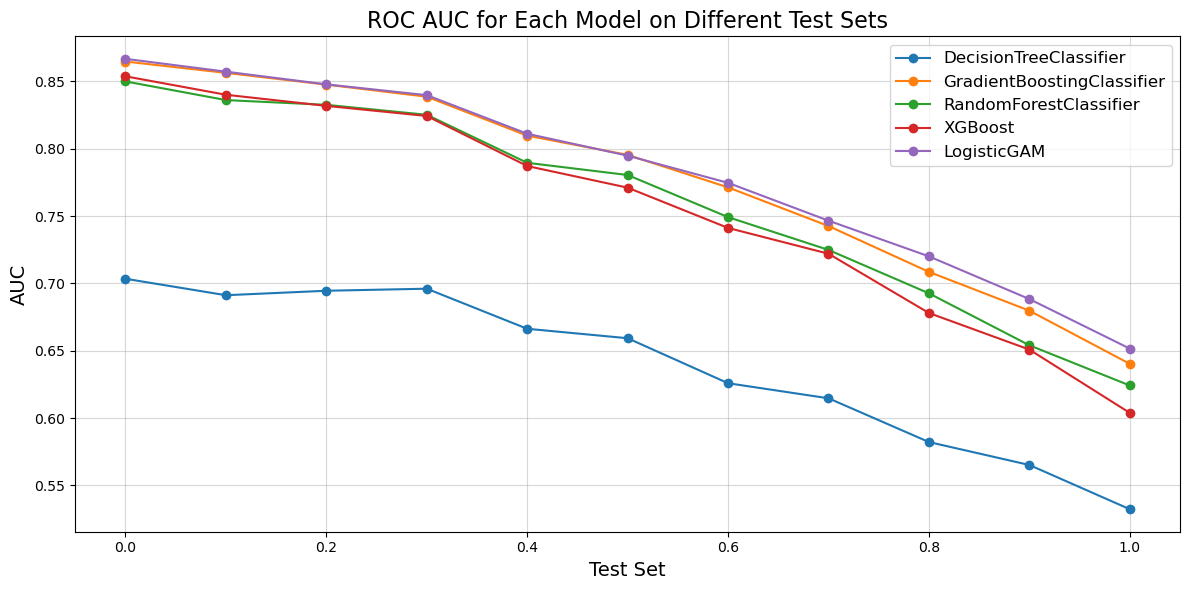
\includegraphics[width=0.8\textwidth]{assets/vanilla.png} 
    \caption{\textbf{Performance of vanilla models on datasets with varying degrees of covariate shift.} The AUC scores of the models are plotted against the mixing probability $p$, which represents the proportion of shifted data in the test set.}
    \label{fig:vanilla-models-perf}
\end{figure}

As we can see from the plot, at low levels of mixed data, the models can still perform realatively well. However, as the proportion of mixed data increases, the performance of the models degrades significantly. The decision tree model is the most sensitive to covariate shift, while the GAM model is the most robust.

Given these preliminary results, we proceeded with hyperparameter optimization to potentially enhance model performance.

\subsubsection{Fine Tuning}

The best choice for hyperparameters in this models might be different depending on the dataset. In order to find the hyperparameters that best fit the data, we performed a hyperparameter tuning using the \plaintt{GridSearchCv} function from the \plaintt{scikit-learn} library, wich performs a cross-validation (k=5) to select the best hyperparameters for each model.

\begin{figure}[H]
    \centering
    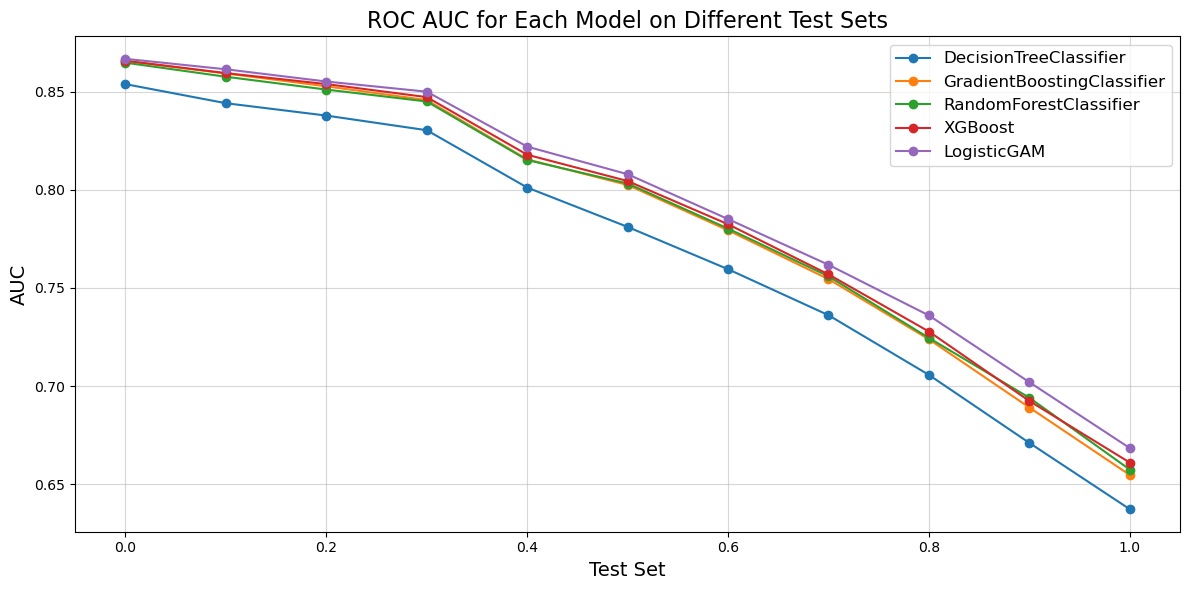
\includegraphics[width=0.8\textwidth]{assets/tuned.png} 
    \caption{\textbf{Performance of fine tuned models on datasets with varying degrees of covariate shift.}}
    \label{fig:tuned-models-perf}
\end{figure}

As shown in \cref{fig:tuned-models-perf}, the fine-tuned models exhibit improved performance compared to the vanilla models. The decision tree model, which was the most sensitive to covariate shift, now performs almost on par with the other models. The GAM model remains the most robust, with consistently high AUC scores across all mixing probabilities.
Bear in mind that we are still working on the fine tuning, expecially for the XGBoost model which uses different methods to perform hyperparameter optimization.

\subsubsection{Overfitting}

% add a brief explanation of why we overfit the models

In order to overfit the models, we created a custom script to perform grid search withot cross-validation. We favored the hyperparameters that achieved the highest score on the training set, while ignoring the necessary precaution to avoid overfitting, i.e. we overshot the maximum depth reachable by the trees.

%Since the logistic GAM is a method which automatically selects the functions that best fit the data, we did not perform any overfitting on it. 
Since the logistic GAM uses different methods to perform fine tuning from the other ones, we are still trying to figure out how to implement a proper overfit. The results for the other models are shown in \cref{fig:overfitted-models-perf}.

\begin{figure}[H]
    \centering
    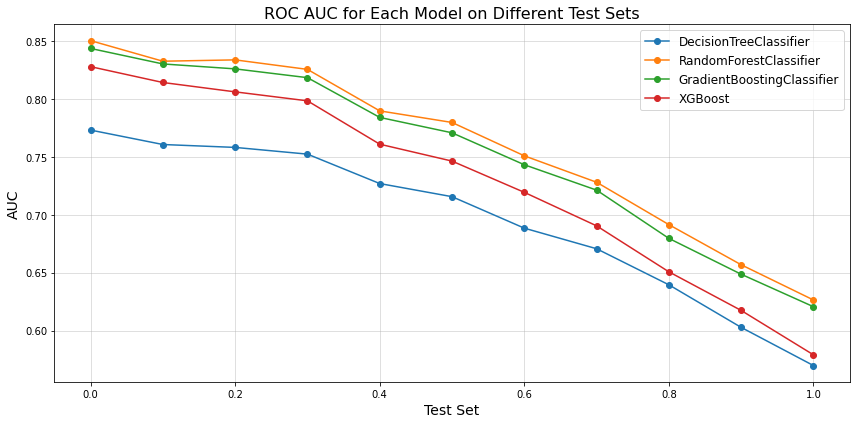
\includegraphics[width=0.8\textwidth]{assets/overfit_no_gam.png} 
    \caption{\textbf{Performance of overfitted models on datasets with varying degrees of covariate shift.}}
    \label{fig:overfitted-models-perf}
\end{figure}


% Although the GAM does not appear to be suffering from overfitting,
As shown in \cref{fig:overfitted-models-perf}, we can clearly see that as we go through increasing percentage of mixed data points, the performance of the models are not on par with the ones that were fine tuned. As the plot further points out, the overfit led to a diversification in the models' AUC scores, with the decision tree model being the most affected by the overfitting process. 